\begin{frame}
\frametitle{Justificación de aplicación de la heurística}

\begin{columns}
\column{0.5\textwidth}
... 

\begin{itemize}

\item Psicología
\item Matemáticas
\item Termodinámica
\item Ciencias de la Computación:
\begin{itemize}

\item ¿Existe una estrategia para jugar en un tiempo indeterminado? 
\item ¿Cuál es la mejor estrategia de juego?
\item \textcolor<1>{red}{¿Existe alguna manera eficiente y automatizada de jugar Tetris?}
{\onslide<2->}
\item \textcolor{red}{¿A qué clase (\textsl{P, NP, NP}-duro o \textsl{NP}-completo) pertenece Tetris?} 
{\onslide}
\end{itemize}

\end{itemize}

\column{0.5\textwidth}
\begin{figure}
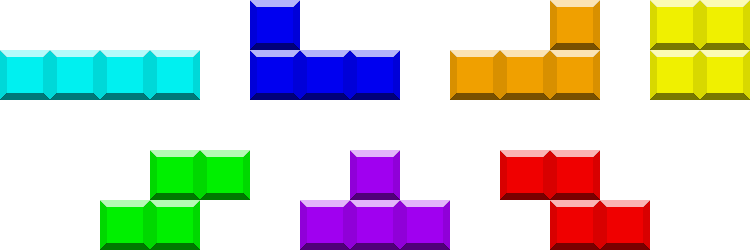
\includegraphics[scale=0.4]{./images/tetrominos.pdf}
\caption{Las piezas de Tetris.}
\end{figure}
\end{columns}

\end{frame}


\begin{frame}
\frametitle{Clasificación de \texttt{TETRIS}}
\pause
\begin{itemize}
\item Formalización del juego:
\begin{itemize}
\pause
\item Tablero: matriz de $n$ por $m$ filas.
\pause
\item Piezas: $P = \langle t, o, \langle i,j \rangle, f \rangle$.
\pause
\item Rotación: $R: \langle P, \theta, B \rangle \mapsto P'$.
\pause
\item Reglas del juego: 
\pause
\begin{itemize}
\item $R(P, 90^{\circ}, B)$.
\item $R(P, -90^{\circ}, B)$.
\item $P' = \langle t, o, \langle i - 1,j \rangle, \texttt{MOVIBLE}\rangle$.
\item $P' = \langle t, o, \langle i + 1,j \rangle, \texttt{MOVIBLE}\rangle$.
\item $P' = \langle t, o, \langle i,j - 1 \rangle, \texttt{MOVIBLE}\rangle$.
\item $P' = \langle t, o, \langle i,j \rangle, \texttt{FIJO}\rangle$.
\end{itemize}
\end{itemize}
\pause
\item \texttt{TETRIS}:
\begin{itemize}

\item \textbf{Input:} Un juego de Tetris de la forma 
$\mathcal{G} = \langle B, P_{1}, P_{2}, ..., P_{p} \rangle$.

\item \textbf{Output:} ¿Existe la secuencia de trayectorias $\Sigma$ tal que 
$\Phi(\mathcal{G}, \Sigma)$ no resulte en una partida perdida?

\end{itemize}
\pause
\item Demostración: ¿Es \texttt{TETRIS} \textsl{NP}? \buonslide[red][1pt]<10->{¿Es \texttt{TETRIS} \textsl{NP}-duro?} {\onslide<11->} $\longrightarrow$ Es \texttt{TETRIS} \textsl{NP}-completo.	
{\onslide}
\end{itemize}
\end{frame}